% !TeX spellcheck = pl_PL
\chapter{Śledzenie obiektów}
\label{cha:sledzenieObiektow}

Śledzenie obiektów polega na określeniu położenia śledzonego obiektu w kolejnych klatkach obrazu określonego materiału wideo. Uzyskana w ten sposób informacja może pomóc m.in. w rozpoznawaniu zachowania ludzi (całych sylwetek bądź twarzy), weryfikacji działania urządzenia przemysłowego czy sterowania pojazdem - czego przykład został opisany w niniejszej pracy.

%---------------------------------------------------------------------------

\section{Rodzaje algorytmów śledzących}
\label{sec:algorytmySledzace}

Algorytmy śledzenia można umieścić w 4 głównych kategoriach utworzonych ze względu na metodę identyfikacji śledzonego obiektu na obrazie. Wyróżnia się algorytmy:
\begin{itemize}
	\item różnicowe
	\item częstotliwościowe
	\item gradientowe
	\item korelacyjne
\end{itemize}

Ponadto, istnieje jeszcze jeden podział podyktowany położeniem kamery względem sceny. W przeciwieństwie do urządzenia o zmiennej pozycji i orientacji w przestrzeni, wykorzystanie kamery stacjonarnej jest stosunkowo proste w realizacji i nie wymaga dużego nakładu obliczeniowego (do głównych czynności należy separacja tła i segmentacja obiektów ruchomych). W przypadku kamery posiadającej stopnie swobody, pomiędzy obecną i kolejną klatką obrazu zmianie ulec mogą wszystkie piksele. Wyklucza to stosowanie algorytmów opartych o wyodrębnianie tła. Dodatkowo, jakikolwiek ruch kamery  znacznie szybciej zmienia położenie obiektu i jego wielkość na obrazie - wymusza to wybór zdecydowanie bardziej złożonych obliczeniowo metod.

\subsection{Algorytmy różnicowe}
Jest to grupa metod, które działają w oparciu o obraz różnicowy, powstały w wyniku odjęcia bieżącego obrazu od poprzedniej klatki lub wcześniej wygenerowanego tła. Pozwala to na wyodrębnienie obszarów, gdzie nastąpiła zmiana, czyli możliwy był ruch. W celu wyeliminowania szumu (minimalnych zmian w wartościach pikseli) stosuje się progowanie, wyjściem z którego jest obraz o pikselach niezmienionych (0) i zmienionych (1). Analizując taką informację, możliwe jest wyznaczenie nowego położenia obiektu i zdefiniowanie przesunięcia, które nastąpiło pomiędzy klatkami. 

Największą zaletą metod różnicowych jest ich prostota w zrozumieniu oraz implementacji, mająca również efekt w niskiej złożoności obliczeniowej. Z drugiej jednak strony, tak proste metody bywają zawodne w przypadku większych zakłóceń i ruchu w sąsiedztwie obiektu, błędnie interpretowanego jako właściwe przesunięcie. Ponadto, zastosowania tych metod ograniczają się jedynie do obrazów rejestrowanych za pomocą kamery stacjonarnej, co eliminuje je z dalszych rozważań w tej pracy. 

\subsection{Algorytmy częstotliwościowe}
Metody te operają się na interpretacji obrazu w dziedzinie częstotliwości. Istnieją różne filtry częstotliwościowe, które pozwalają na wykrycie krawędzi - więc, odpowiednio zaimplementowane, umożliwiają również identyfikację obiektu dla kolejnych klatek wideo. Przykładem takiej metody jest filtr Gabora, który koncentruje się na informacji o teksturze, nie na kolorze. Praca w dziedzinie częstotliwości daje możliwość wykrycia przesunięć obiektu, które mogłyby zostać niezauważone w przypadku stosowania pozostałych typów metod. Swoją wysoką dokładność algorytmy te każą jednak opłacać nieporównywalnie większą złożonością obliczeniową, związaną z obliczeniem transformaty Fouriera i stosowaniem filtrów częstotliwościowych.

\subsection{Algorytmy gradientowe}
Działanie wspomnianych metod śledzenia obiektów opiera się na założeniu niewielkich zmian w luminancji (jasności, oświetleniu) oraz przesunięciu obiektu pomiędzy kolejnymi klatkami obrazu. Istotą tych algorytmów jest znalezienie odpowiedniego przesunięcia obiektu pomiędzy kolejnymi klatkami, tak, aby wskaźnik jakości wynikający z podobieństwa obszarów był zminimalizowany. Poszukiwania obszaru można realizować globalnie, bądź na fragmencie będącym otoczeniem śledzonego obiektu. Algorytm prowadzący obliczenia lokalnie może zawodzić w sytuacjach, gdy przesunięcia są zbyt duże i wykraczają poza obszar poszukiwań, jednak taka metodyka obniża złożoność obliczeniową całego algorytmu i znajduje swoje zastosowania w określonych sytuacjach. Spośród wielu algorytmów gradientowych stosowanych do śledzenia obiektów, najpopularniejszymi są MeanShift, Camshift oraz HOG.

\subsection{Algorytmy korelacyjne}
Algorytmy te wyznaczają korelację bloków pikseli i dążą do maksymalizacji funkcji korelacyjnej. Działają zgodnie z założeniem, że istnieje jeden wspólny kierunek przemieszczenia wszystkich punktów obiektu, nie są zatem najlepszym rozwiązaniem dla innych typów ruchu. Istotnym parametrem przy implementacji tej grupy metod jest określenie rozmiaru obszaru poszukiwań - w przypadku mniejszych, problemem bywa przemieszczenie obiektu poza obszar; w przypadku większych istnieje ryzyko znalezienia maksimum funkcji korelacyjnej, które nie odpowiada obiektowi. Zaletą metod korelacyjnych jest jednak możliwość wyboru ilości i dowolnego rozmieszczenia wektorów ruchu. Stosuje się je często, gdy obliczanie pochodnych (dla metod gradientowych) byłoby utrudnione - przykładowo w przypadku gwałtownego ruchu obiektu lub niewystarczającej wielkości klatkażu w materiale wideo.

\subsection{Podsumowanie}
Ostatecznie w realizacji projektu postanowiono zaimplementować algorytmy gradientowe: MeanShift i HoG/SVM. O takim wyborze zadecydowała możliwość wykorzystania algorytmów dla obrazu pochodzącego z kamery ruchomej, co w przypadku pracy drona było decyzją naturalną. Mimo, że MeanShift jest algorytmem iteracyjnym (kryterium zakończenia obliczeń stanowi limit iteracji bądź uzyskanie określonej dokładności), można stwierdzić, że implementacja w układzie FPGA pozwoli przetwarzać obraz w czasie rzeczywistym, tj. ukończyć przetwarzanie aktualnej klatki przed rozpoczęciem przetwarzania kolejnej tak szybko jak tylko uzyska się na jej temat komplet informacji. Metoda ta charakteryzuje się dobrymi wynikami w przypadku obiektów zmieniających orientację - jest to szczególnie przydatne w sytuacji, gdy miejscem umiejscowienia kamery jest dron - maszyna podatna na podmuchy zmieniające chwilowo jego orientację względem obiektu. Z kolei wsparcie algorytmem HoG/SVM będzie szczególnie przydatne w kompensowaniu głębi, czyli oddalenia maszyny od obiektu. Poprawność działania systemu wbudowanego będącego połączeniem obu algorytmów została potwierdzona testami, które zostały przeprowadzone na modelu programowym oraz na symulacjach kodu System Verilog.

\section{Algorytm MeanShift}

\subsection{Konwersja przestrzeni barw RGB->HSV}
\label{fig:HSV_cone}
Algorytm MeanShift użyty w procesie śledzenia wykorzystuje rozkład prawdopodobieństwa wybranej cechy na obrazie - w tym wypadku barwy. Jest to składowa H z przestrzeni barw HSV (ang. Hue, Saturation, Value). Domyślną przestrzenią do rejestracji i zapisu obrazów jest jednak RGB, zatem wymagana jest jej konwersja. O ile przestrzeń RGB reprezentowana jest przez sześcian określony parametrami 3 kolorów: czerwonego, zielonego i niebieskiego, to przestrzeń barw HSV opisywana jest przez stożek. Jego podstawą jest koło barw, którego kąt opisuje odcień światła (H - Hue). Kolor czerwony jest reprezentowany przez kąty 0\si{\degree} (lub 360\si{\degree}), zielony przez kąt 120\si{\degree}, a kolor niebieski przez 240\si{\degree}. Promień koła barw opisuje nasycenie koloru (S - Saturation), zaś za moc światła białego, czyli jasność (V - Value) odpowiada wysokość stożka. Model HSV jest lepiej powiązany ze sposobem, w jaki postrzega ludzki narząd wzroku, dla którego wszystkie barwy są światłem odbitym od obiektów. Rysunek \ref{fig:HSV_cone} przedstawia interpretację graficzną składowych przestrzeni HSV na stożku.

\begin{figure}[h]
	\centering
	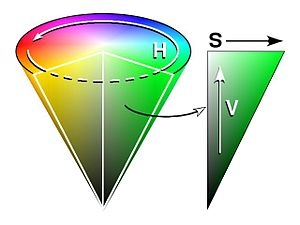
\includegraphics[width=6cm]{2_HSV.jpg}
	\caption{Stożkowa przestrzeń barw modelu HSV}
	\label{fig:HSV_cone}
\end{figure}

Poniższe wzory opisują sposób wyznaczenia poszczególnych składowych przestrzeni HSV w oparciu o RGB:

\begin{equation}
\label{HSV_first}
V=max(R,G,B)
\end{equation}

\begin{equation}
S=\begin{cases}
\frac{V-min(R,G,B)}{V}, & V\neq0 \\
0, & V=0
\end{cases}
\end{equation}

\begin{equation}
\label{HSV_last}
H=\begin{cases}
	0, & \text{jeśli } V-min(R,G,B)==0 \\
	\frac{60(G-B)}{V-min(R,G,B)}, & \text{jeśli } V==R \\
	\frac{60(B-R)}{V-min(R,G,B)}+120, & \text{jeśli } V==G \\
	\frac{60(R-G)}{V-min(R,G,B)}+240, & \text{jeśli } V==B 
\end{cases}
\end{equation}

\subsection{Wektor MeanShift}
\label{ssec:MS}
Istotą działania algorytmu MeanShift jest wyznaczanie maksimum funkcji gęstości w kolejnych iteracjach. Dla określanego obszaru obliczany jest środek masy punktów, do którego po zakończeniu algorytmu jest przesuwane aktualne położenie środka. To przesunięcie nosi nazwę \textit{wektora MeanShift}, który dla zbioru \textit{n} punktów $\{x_{i}\}_{i=1..n}$ oraz środka obszaru w punkcie $y_0$ może zostać zapisany jako:

\begin{equation}
\label{eq:ms1}
M(y)=\bigg[\frac{1}{n}\mathlarger{\sum\limits_{i=1}^{n}}x_i\bigg]-y_0
\end{equation}

Prostota wzoru \ref{eq:ms1} wynika z ujednolicenia wagi dla wszystkich punktów. Wprowadzając wagę punktu zależną od jego odległości od środka obszaru - takiej, która maleje wraz z oddalaniem się od centrum), wzór \ref{eq:ms1} można przepisać jako:

\begin{equation}
\label{eq:ms2}
M(y)=\frac{\sum_{i=1}^{n}w_i(y_0)x_i}{\sum_{i=1}^{n}w_i(y_0)}-y_0
\end{equation}
W równaniu \ref{eq:ms2}, $w_i(y_0)$ są wagami dla poszczególnych punktów.

Rysunek  \ref{fig:ms_vector} ilustruje przykładowe wygenerowanie wektora MeanShift, gdzie niebieskim okręgiem zaznaczono obszar podlegający działaniu algorytmu. Wszystkie punkty mają tu jednak identyczną wagę.
\begin{figure}[h]
	\centering
	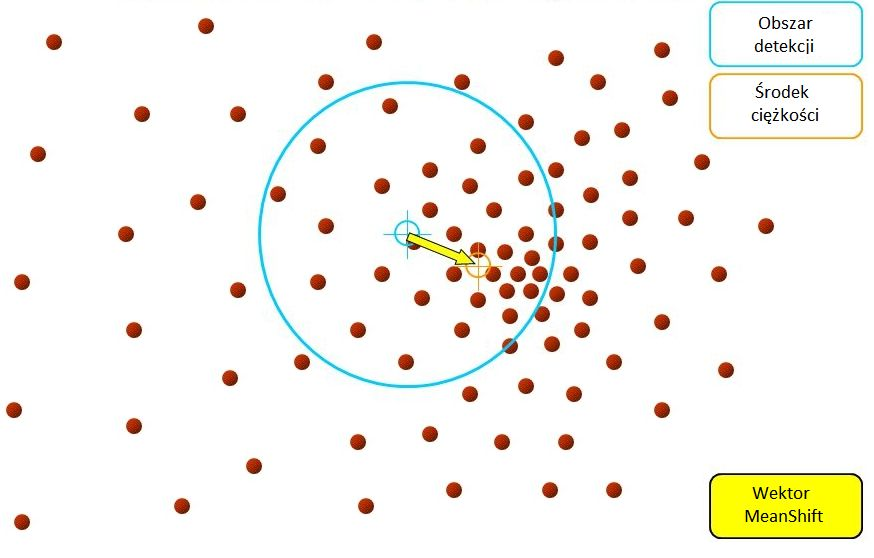
\includegraphics[width=10cm]{2_meanshift.jpg}
	\caption{Graficzna interpretacja wektora MeanShift \cite{Egorov}}
	\label{fig:ms_vector}
\end{figure}

\subsection{Jądro obszaru}
Celem wyznaczenia jądra (ang. \textit{kernel}) dla obszaru o stałej wielkości jest przypisanie najwyższej wagi punktom, które znajdują się najbliżej środka obszaru. Konsekwencją tego jest nadawanie znikomych wag punktom na jego rubieżach. Postać jądra zwykle przyjmuje klasyczne postacie gęstości rozkładów probabilistycznych: między innymi rozkładu jednorodnego (wagi jednakowe), prostokątnego, Gaussa, Cauchy'ego, Epanechnikova. W niniejszej pracy zdecydowano się wykorzystać jądro trójkątne ze względu na jego dobre wyniki i jednoczesną prostotę implementacji, nie bez znaczenia podczas późniejszej ealizacji sprzętowej w układzie FPGA. Jądro takie można opisać poniższym wzorem:

\begin{equation}
\label{eq:ms3}
K(u)=\begin{cases}
1-\frac{u}{b}, & \text{jeśli }\frac{u}{b}\leq 1 \\
0, & \text{jeśli }\frac{u}{b} > 1
\end{cases}
\end{equation}
gdzie $u$ jest odległością pomiędzy punktem a środkiem obszaru, a $b$ jest połową jego boku (zakładając, że obszarem jest kwadrat). Rysunek \ref{fig:kernel} przedstawia jądro o wymiarach 100x100 - w punkcie (50,50) osiąga maksymalną wartość 1 (natomiast $u=0$).
\begin{figure}[h]
	\centering
	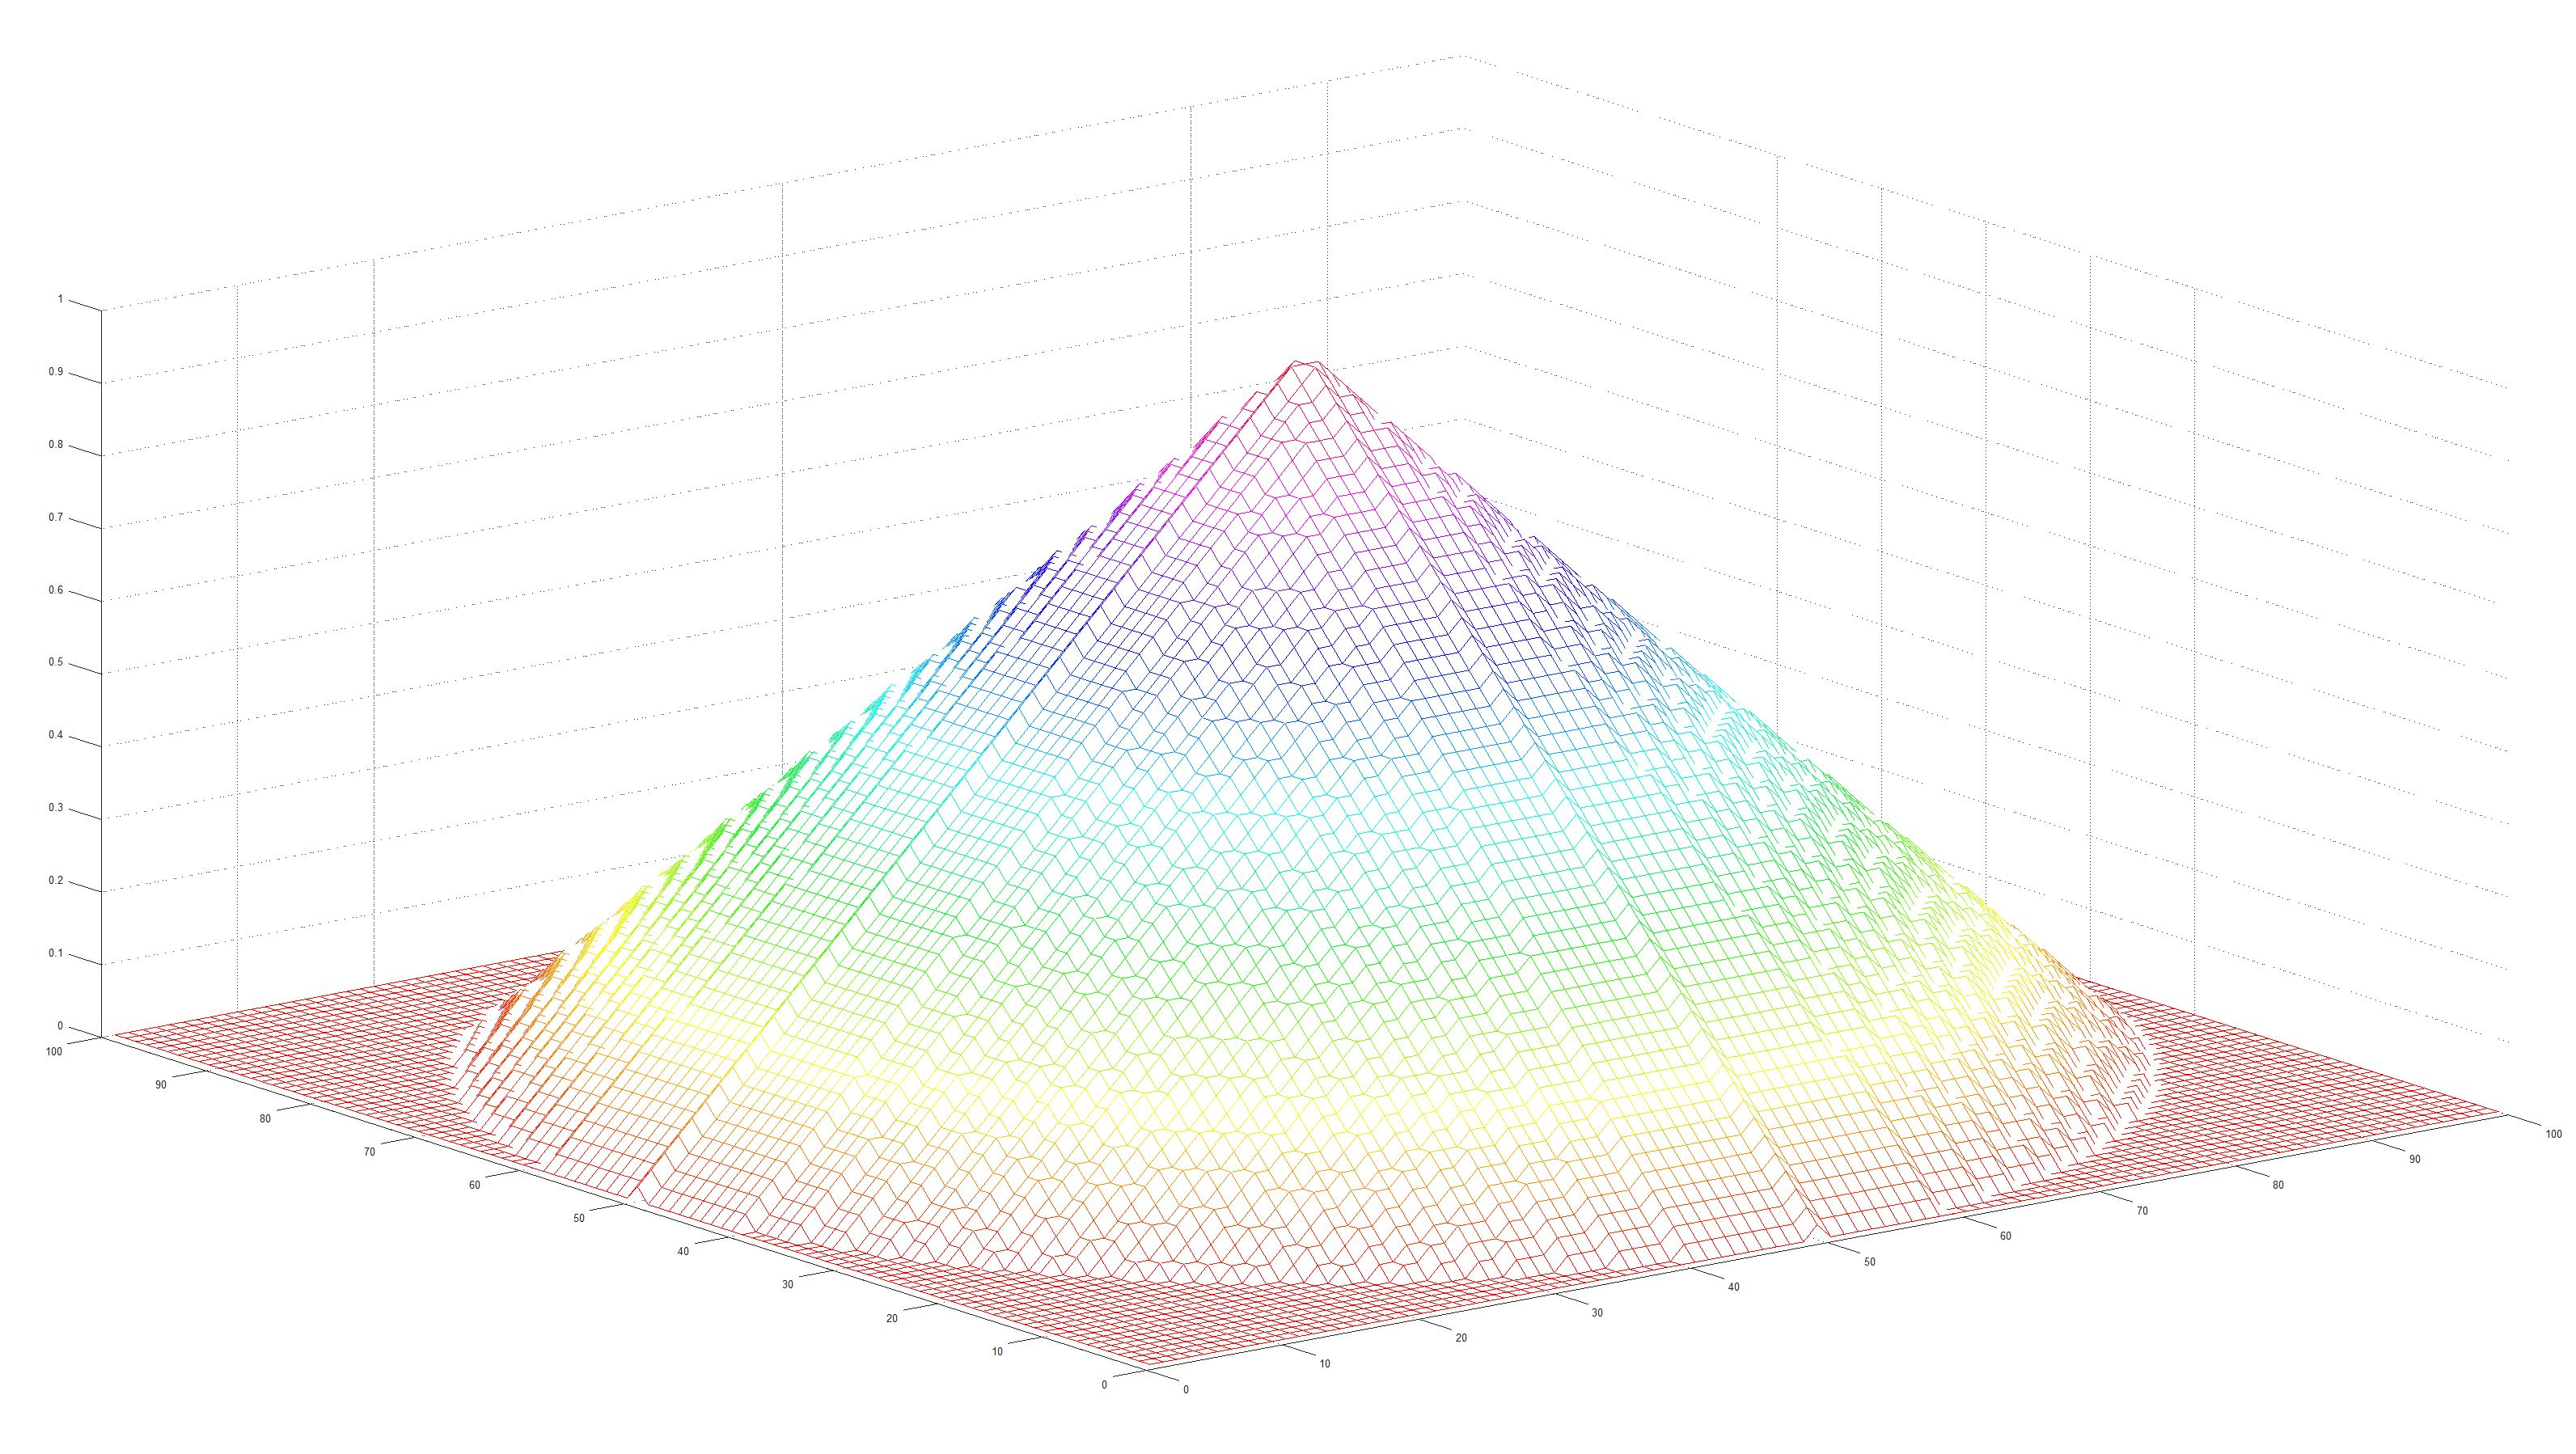
\includegraphics[width=16cm]{2_kernel.jpg}
	\caption{Jądro obszaru o wymiarach 100x100 (wygenerowane w programie MATLAB)}
	\label{fig:kernel}
\end{figure}

\subsection{Gęstość jądra}
Mając zbiór $n\times n$ punktów: $\{x_{i},y_{j}\}_{i=1..n,i=j..n}$ z przestrzeni $\mathbb{R}^2$ oraz jądro $K(u)$ dla punktu centralnego $P=(x,y)$ można przedstawić funkcję oszacowania gęstości:

\begin{equation}
\left.\begin{aligned}
f(P)&=\frac{1}{n^2}\sum_{i=1}^{n}\sum_{j=1}^{n}K(P-P'(i,j)) \\
f(P)&=\frac{1}{n^2}\sum_{i=1}^{n}\sum_{j=1}^{n}K(||P-P'(i,j)||).
\end{aligned}\right.
\end{equation}
Różniczkując powyższe otrzymuje się:
\begin{equation}
\label{eq:K}
\nabla f(P)=\frac{1}{n^2}\sum_{i=1}^{n}\sum_{j=1}^{n}(P-P'(i,j))K'(||P-P'(i,j)||),
\end{equation}
a po podstawieniu $g(x)$ za $-K'(x)$, wzór \ref{eq:K} może zostać zapisany jako:
\begin{equation}
\nabla f(x)=\frac{1}{n^2}\sum_{i=1}^{n}(P-P'(i,j))g(||P-P'(i,j)||),
\end{equation}
Po przekształceniu wzór może być przedstawiony jako:
\begin{equation}
\label{eq:kerms}
\begin{aligned}
\nabla f(x)= &\frac{1}{n^2}\bigg[\sum_{i=1}^{n}\sum_{j=1}^{n}g(||P-P'(i,j)||)\bigg] \cdot\\ \cdot&\bigg[\frac{\sum_{i=1}^{n}\sum_{j=1}^{n}P'(i,j)g(||P-P'(i,j)||)}{\sum_{i=1}^{n}\sum_{j=1}^{n}g(||P-P'(i,j)||)} -P\bigg],
\end{aligned}
\end{equation}
Ze wzoru \ref{eq:kerms} można wyodrębnić człon będący gradientem jądra: $g(P)=-K'(P)$. Drugą jego część stanowi wektor MeanShift z wagami odpowiadającymi wartościom gradientu jądra o środku w punkcie $x$. Zakładając niezerowość wyrażenia $\sum_{i=1}^{n}\sum_{j=1}^{n}g(||P-P'(i,j)||^2)$, wektor ten może przyjąć ostateczną formę:
\begin{equation}
M_s(P)=\frac{\sum_{i=1}^{n}\sum_{j=1}^{n}P'(i,j)g(||P-P'(i,j)||)}{\sum_{i=1}^{n}\sum_{j=1}^{n}g(||P-P'(i,j)||)} -P.
\end{equation}

\subsection{Współczynnik Bhattacharyya}
 \label{ssec:Bhat}
Zastosowanie algorytmu MeanShift do śledzenia obiektów na materiale
wideo wymaga znalezienia zależności pomiędzy funkcjami gęstości wzorca oraz kandydata. W tym celu należy zestawić ze sobą oba rozkłady na przykład za pomocą współczynnika Bhattacharyya, który dla $m$-wymiarowych funkcji gęstości wzorca $q_h$ oraz obszaru-kandydata $p_h$ ze środkiem w punkcie $P$ wyraża się wzorem:
\begin{equation}
\label{eq:Bhat}
\rho(P)=\sum_{h=1}^{m}\sqrt{p_h(P)q_h}
\end{equation}
Wyznaczenie przesunięcia obiektu na obrazie dla kolejnych klatek obrazu wymaga znalezienia maksymalnego współczynnika Bhattacharyya, co jest tożsame (według algorytmu) ze zidentyfikowaniem najbardziej podobnego fragmentu do oryginalnego obszaru śledzonego.

\subsection{Śledzenie}
Opisane wyżej jądro i jego gradient stanowią inicjalizację całego algorytmu i są obliczane jeszcze przed zdefiniowaniem wzorca. Cechą obrazu, dla której będzie liczona funkcja prawdopodobieństwa, jest kolor (H z przestrzeni barw HSV, jest to liczba z zakresu 0-359). 
Jeśli położenie piksela na obrazie wzorca oznaczone jest jako $\{x_{i},y_{j}\}_{i=1..n,i=j..n}$, niech zdefiniowana będzie funkcja $b:\mathbb{R}^2\rightarrow\{1..m\}$, która odwoływać się będzie do składowej \textit{H} danego piksela.

Barwa piksela jest przede wszystkim argumentem funkcji prawdopodobieństwa utworzonego dla \textit{H} na danym obszarze detekcji. Współczynnik Bhattacharyya jest \textit{de facto} porównaniem dwóch funkcji prawdopodobieństwa (wzorca i kandydata) o wymiarze cech równym 360.   
Podczas obliczania prawdopodobieństwa wystąpienia określonego koloru, istotną rolę odgrywać musi wartość jądra, które zwiększa wagę pikseli znajdujących się w centrum obszaru, marginalizując znaczenie tych brzegowych - które mogłyby być częścią zmiennego w czasie tła. O ile w tradycyjnym histogramie wartości przedziałów zwiększa się poprzez inkrementację, to w tym przypadku zdecydowano się na powiększenie o wartość jądra odpowiadającego położeniu piksela na obszarze 100x100.
 Dla przykładowej barwy $h$, funkcja gęstości prawdopodobieństwa może być zdefiniowana jako:
\begin{equation}
q_h=C\sum_{i=1}^{n}\sum_{j=1}^{n}K(||P-P'(i,j)||)\delta[b(P'(i,j))-h],
\end{equation}
gdzie $P$ to nadal środek obszaru detekcji a symbol $\delta$ jest deltą Kroneckera. Współczynnik $C$ odpowiada za normalizację $q_h$: $\sum_{h=1}^{m}q_h=1$.
Po przekształceniu okazuje się, że:

\begin{equation}
C=\frac{1}{\sum_{i=1}^{n}\sum_{j=1}^{n}K(||P-P'(i,j)||)} 
\end{equation}

W każdej iteracji dla kandydata wyznacza się funkcję gęstości prawdopodobieństwa. Uwzględniając obszar ze środkiem w punkcie $P$, wzór prezentuje się następująco:
\begin{equation}
\label{eq:density}
p_h(P)=C_k\sum_{i=1}^{n}\sum_{j=1}^{n}K(||P-P'(i,j)||)\delta[b(P'(i,j))-h] 
\end{equation}

Współczynnik $C_h$ wyznacza się podobnie, jak dla wzorca, jednak z uwgzlędnieniem położenia środka obszaru kandydata, $P$:
\begin{equation}
C_k=\frac{1}{\sum_{i=1}^{n}\sum_{j=1}^{n}K(||P-P'(i,j)||)} 
\end{equation}
Następnie należy zbadać podobieństwo obu rozkładów gęstości - wykorzystywany jest w tym celu współczynnik Bhattacharyya, opisany w rozdziale \ref{ssec:Bhat}. Rozwijając wzór \ref{eq:Bhat} w szereg Taylora ze środkiem obszaru wzorca równym $P_0$ można otrzymać:
\begin{equation}
\label{eq:approx}
\rho(p(P),q)\approx\frac{1}{2}\sum_{u=1}^{m}\sqrt{p_u(P_0)q_u} + \frac{1}{2}\sum_{u=1}^{m}p_u(P)\sqrt{\frac{q_u}{p_u(P_0)}}
\end{equation}
Podstawienie równania \ref{eq:density} do powyższego wyrażenia daje:
\begin{equation}
\label{similarity_est}
\begin{aligned}
\rho(p(P),q)\approx & \frac{1}{2}\sum_{u=1}^{m}\sqrt{p_u(P_0)q_u} + \\ & \frac{C_k}{2}\sum_{i=1}^{n}\sum_{j=1}^{n}\sum_{u=1}^{m}\sqrt{\frac{q_u}{p_u(P_0)}}\delta[b(P'(i,j))-h] k(||P-P'(i,j)||)
\end{aligned}
\end{equation}
Stąd można wyodrębnić:
\begin{equation}
\label{eq:wi}
w_{i,j}=\sum_{u=1}^{m}\sqrt{\frac{q_u}{p_u(P_0)}}\delta[b(P'(i,j))-h]
\end{equation}


We wzorze \ref{similarity_est} pierwsza składowa jest niezależna od położenia środka obszaru kandydata $P$. Maksymalizując funkcję podobieństwa, należy skupić się na poszukiwaniu największej wartości drugiego członu. 
Wykorzystując wektor MeanShift z rozdziału \ref{ssec:MS} z wagami równymi wartościom funkcji podobieństwa wzorca i kandydata oraz wzór \ref{eq:wi}, dla każdej klatki obrazu i w każdej iteracji należy wyliczyć aktualne położenie obszaru w oparciu o względne przesunięcie dane poniższym wzorem.

\begin{equation}
\label{eq:position}
\Delta P=\frac{\sum_{i=1}^{n}\sum_{j=1}^{n}P(i,j)\cdot w_{i,j}\cdot g(P-P'(i,j))}{\sum_{i=1}^{n}\sum_{j=1}^{n}w_{i,j}\cdot g(||P-P'(i,j)||)}
\end{equation}

\subsection{Warunki zakończenia algorytmu}
W przypadku algorytmu iteracyjnego konieczne jest zdefiniowanie celów, które należy osiągnąć. Uzyskanie całkowitego podobieństwa pomiędzy wzorcem i kandydatem w zmiennej sekwencji obrazów raczej nie jest do osiągnięcia. Chcąc przetwarzać obraz w czasie rzeczywistym, należy zakończyć przetwarzanie klatki przed momentem, w którym dane z następnej będą gotowe. Stąd dwa podstawowe warunki zakończenia algorytmu to:
\begin{enumerate}
	\item numer iteracji == maksymalna liczba iteracji
	\item $||y_{n_m}-y_{n_{m-1}}||==0$,
\end{enumerate} 
gdzie $n$ jest liczbą porządkową klatki, a $m$ jest numerem iteracji algorytmu MeanShift dla konkretnej klatki.
W momencie spełnienia jednego z powyższych warunków, akceptuje się dotychczasowo uzyskaną zmianę położenia obszaru detekcji i rozpoczyna obliczenia następnej klatki. \newline Rysunek \ref{fig:MS_diagram} przedstawia diagram algorytmu MeanShift dla sygnału wideo.
\begin{figure}
	\centering
	\hspace*{-3cm}
	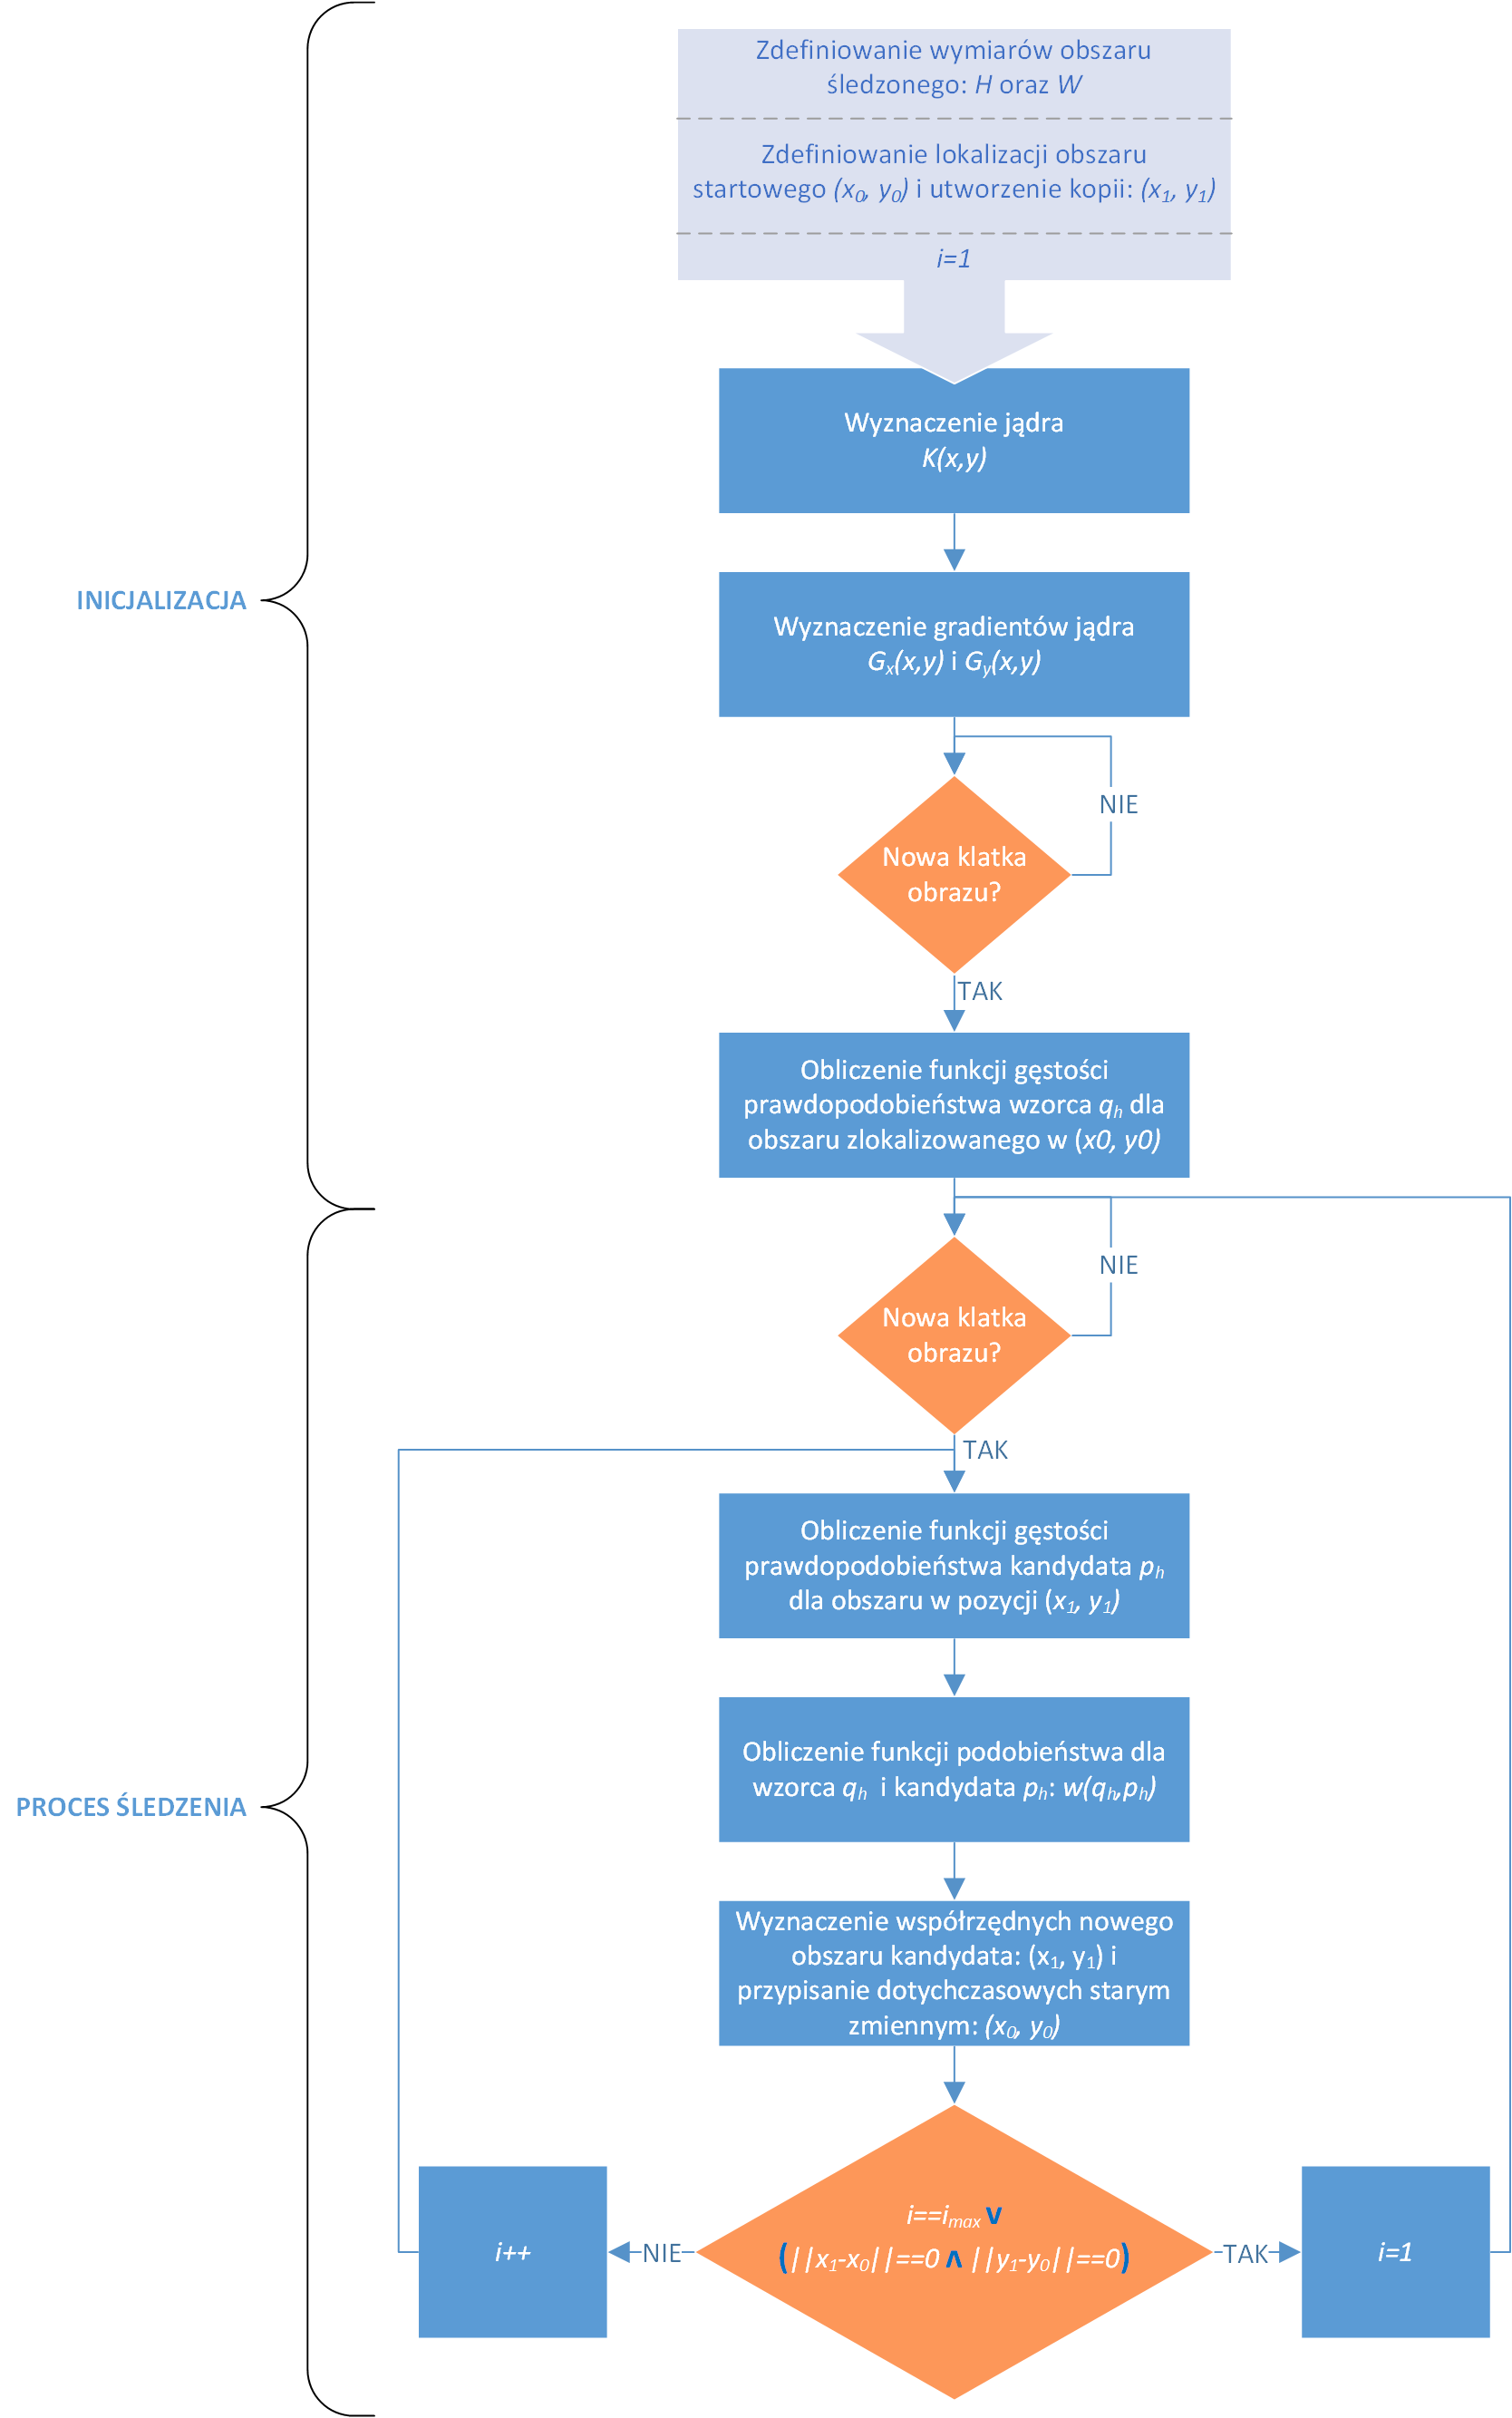
\includegraphics[width=14.5cm]{2_MS_visio.png}
	\caption{Schemat blokowy algorytmu MeanShift}
	\label{fig:MS_diagram}
\end{figure}

\section{Algorytm HOG+SVM}
\label{sec:HOG&SVM}
Inną gradientową metodą detekcji (oraz śledzenia) jest algorytm wykorzystujący zestaw cech obrazu - konkretnie histogram ukierunkowanych gradientów (ang. \textit{Histogram of Oriented Gradients - HOG}); rolę decyzyjną pełni klasyfikator nazywany maszyną wektorów nośnych (ang. \textit{Support Vector Machine - SVM}). Pierwotnie, ten rodzaj hybrydy został przedstawiony w pracy [Dalal and Triggs, 2005], z zastosowaniem w detekcji pieszych, co może czynić go wystarczająco dopasowanym do potrzeb niniejszego projektu. Oczywiście należy dodać, że dysponując odpowiednim zestawem informacji, odpowiednio trenowany mechanizm SVM byłby w stanie działać z innymi obiektami.

\subsection{Konwersja RGB->GRAY i kąty gradientów}
\label{sec:HOGgrad}
Pierwszym etapem jest dostosowanie pierwotnej palety barw RGB do 8-bitowej skali szarości. Dokonuje się tego, przekształcając każdy piksel według wzoru:
\begin{equation}
\label{eq:rgb2gray}
P_{GRAY}=0.299P_R + 0.587P_G + 0.114P_B 
\end{equation}
Sumowanie się współczynników do jedności ma w zamierzeniu ograniczyć wynik tego przekształcenia do zakresu 0-255.

Następnie przeprowadzana jest operacja kontekstowa w celu obliczenia gradientów kierunkowych $g_x$ oraz $g_y$; używane maski to odpowiednio: $[-1,0,1]$ oraz $[-1,0,1]^T$. 
Mając gradienty, dla każdego piksela (o koordynatach [$i,j$]) obliczany jest także moduł i kąt ze wzorów:

\begin{equation}
\label{eq:HOGangles}
\left.\begin{aligned}
m(i,j)=\sqrt{g_x(i,j)^2+g_y(i,j)^2} \\
\theta(i,j)=arctg\bigg(\frac{g_y(i,j)}{g_x(i,j)}\bigg)
\end{aligned}\right.
\end{equation}

\subsection{Histogram gradientów}
W kolejnym etapie poddawany przetwarzaniu obraz będzie dzielony na kwadratowe obszary (dla jasności nazywane od teraz \textit{komórkami}) o wymiarach 4x4, 8x8 czy 16x16 pikseli. W każdej z komórek zostanie wyliczony niezależny histogram na podstawie kątów gradientu. Oprócz rozmiaru komórki, kluczowym okazuje się również drugi parametr, czyli ilość przedziałów klasowych pojedynczego histogramu - w tym wypadku zdecydowano, by rozpatrywany kąt przyporządkowywać jednemu z 9 przedziałów równo dzielących zakres $[0^{\circ},180^{\circ})$ - i komplementarnie $[-180,0)$. Wynika z tego, że każdy kolejny zakres $a=180/9=20^{\circ}$ będzie stanowić osobny przedział klasowy histogramu.

O ile typowy histogram tworzony jest poprzez inkrementację odpowiedniego przedziału o 1, to tworzona struktura będzie wykorzystywać obliczony wcześniej moduł z gradientu. Dodatkowo, autorzy publikacji wspominają o możliwości interpolacji pomiędzy dwoma sąsiednimi przedziałami i inkrementacji poszczególnych wartości o proporcjonalne części modułu - takie działanie ma pozytywnie wpływać na wyniki detekcji. Jeśli zatem przyjąć, że $\theta_h$ i $\theta_l$ to wartości kątów będących środkami dwóch sąsiadujących ze sobą przedziałów, którym jednocześnie najbliżej do badanego kąta $\theta$, wówczas będzie można zdefiniować inkrementy $M_h$ i $M_l$ jako:

\begin{equation}
\label{eq:HOG_linear}
\left.\begin{aligned}
M_h(i,j)&=m(i,j)\bigg(\frac{\theta-\theta_l}{a}\bigg)\\
M_l(i,j)&=m(i,j)\bigg(\frac{\theta_h-\theta}{a}\bigg)
\end{aligned}\right.
\end{equation}
Ostatecznie, następuje powiększenie wartości dwóch odpowiednich przedziałów histogramu $H$ tworzonego w obrębie komórki zawierającej piksel o współrzędnych (i,j):

\begin{equation}
\label{eq:HOG_increment}
\left.\begin{aligned} 
H(\theta_h,i,j)&=H(\theta_h)+M_h(i,j) \\ 
H(\theta_l,i,j)&=H(\theta_l)+M_l(i,j)
\end{aligned}\right.
\end{equation}

Przykładem może być sytuacja przedstawiona na rysunku \ref{fig:HOG_interpolation}. Wyjątkowym zdarzeniem jest takie, w którym kąt $\theta$ będzie znajdował w okolicy kąta $0^{\circ}=360^{\circ}$ (z przedziałami 1 oraz 9). Wówczas, dla wygody, w równaniach \ref{eq:HOG_linear} należy użyć kątów $\theta_l=350^{\circ}$ oraz $\theta_h=370^{\circ}$.

\begin{figure}[h]
	\centering
	\hspace*{1cm}
	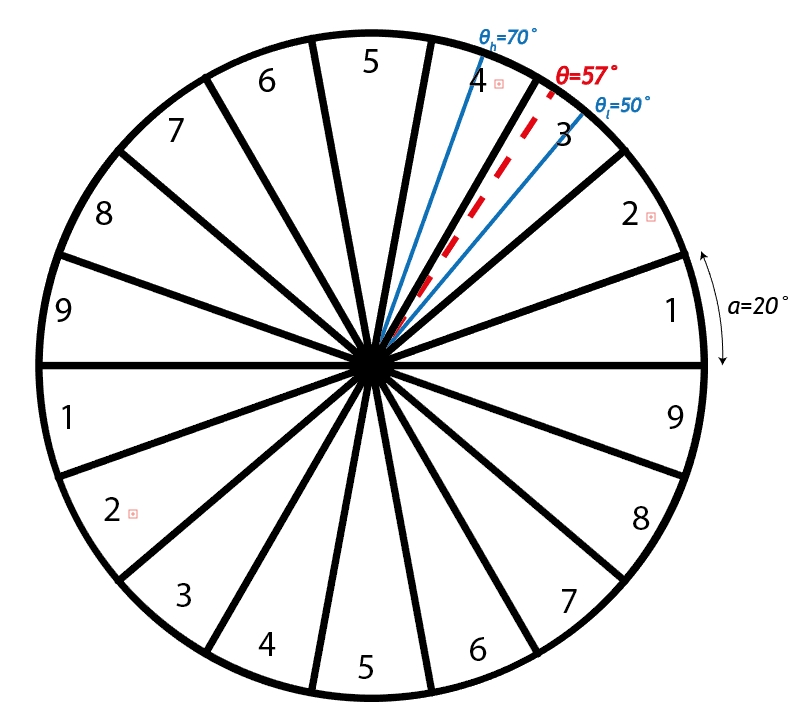
\includegraphics[width=12cm]{2_HOG_interpolation.jpg}
	\caption{Przykładowy problem liniowej interpolacji}
	\label{fig:HOG_interpolation}
\end{figure}

\subsection{Normalizacja}
Zazwyczaj, analizowany materiał wideo będzie nagrywany w amatorskich warunkach, co może w efekcie oznaczać nierówny poziom oświetlenia poszczególnych fragmentów obrazu. Zdegenerowany w ten sposób obraz nie dawałby dobrych wyników działania algorytmu. Z tego powodu proponuje się stosowanie blokowej normalizacji. 

Proponowane podejście zakłada utworzenie struktur nazywanych \textit{blokami}, gdzie każdy z nich obejmować ma $2\times 2$ sąsiednie komórki. Dla obrazu, na bazie którego utworzono $N \times M$ komórek, powinno powstać $N-1 \times M-1$ bloków - przy ich generowaniu wykonuje się krok o jedną komórkę w poziomie i/lub w pionie względem poprzedniego obszaru. Rozmiar pojedynczego bloku sugeruje, że będzie się on składał z 4 histogramów, w formie wektora: 
\begin{equation}
v=[H_{i,j}, H_{i,j+1}, H_{i+1,j}, H_{i+1,j+1}],
\end{equation} 
gdzie $i$  wiersz, $j$ - kolumna. Następnie należy obliczyć wektor cech $L$, wykorzystując jedną z sugerowanych zależności:

\begin{equation}
\label{eq:HOG_norm1}
\left.\begin{aligned} 
L1&=\frac{v}{\sum_{i}^{n}v_i+\epsilon}
\end{aligned}\right.
\end{equation}

\begin{equation}
\label{eq:HOG_norm2}
\left.\begin{aligned} 
L1_{sqrt}&=\frac{v}{\sqrt{\sum_{i}^{n}v_i+\epsilon}}
\end{aligned}\right.
\end{equation}

\begin{equation}
\label{eq:HOG_norm3}
\left.\begin{aligned} 
L2&=\frac{v}{\sqrt{\sum_{i}^{n}v_i^2+\epsilon^2}}
\end{aligned}\right.
\end{equation}

\begin{equation}
\label{eq:HOG_norm4}
\left.\begin{aligned} 
L2_{hys}&=\frac{v}{\sqrt{\sum_{i}^{n}v_i^2+\epsilon^2}}, v\leq 0.2
\end{aligned}\right.
\end{equation}
W powyższych równaniach $\epsilon$ to stała o małej wartości, a $n$ to liczba elementów w bloku (4 histogramy po 9 przedziałów $\rightarrow$ 36). Wektory $L$ zebrane z całego okna detekcji budują ostateczny wektor cech, na którym pracować będzie klasyfikator.

Niech podsumowaniem rozważania będzie przykład - obraz o rozmiarze $720\times 1280$ i komórka o wielkości $8 \times 8$. Wynikiem opisywanej procedury będzie utworzenie aż $90\cdot160=14400$ komórek i $89\cdot 159=14151$ bloków. Po normalizacji, klasyfikator otrzymałby aż $14151\cdot36=509436$ wartości do przetworzenia. Tak duża wartość niosłaby jednak za sobą konieczność optymalizacji, co będzie rozważone w rozdziale poświęconym implementacji algorytmu.

\subsection{Klasyfikator SVM}
Maszyna wektorów nośnych to klasyfikator binarny, który dzięki swej prostocie i skuteczności jest powszechnie wykorzystywany w procesie odróżniania klas. Jego działanie tradycyjnie można podzielić na dwie fazy: uczenie i klasyfikację. \newline Etap uczenia to relatywnie dłuższy czasowo proces wyznaczenia hiperpłaszczyzny, która z jak najlepszym marginesem rozdzieli wejściowe wektory cech obiektów klasyfikowanych jako \textit{1} od tych określonych jako \textit{0} (umownie). Stosowane podeście nie powinno odbiegać od klasycznej metodologii uczenia maszynowego - dysponując zbiorem danych wejściowych, należy dokonać podziału na próbki trenujące oraz testowe (w stosunku około 70:30). Każdy z z tych podzbiorów (a przede wszystkim trenujący) powinien posiadać zarówno obiekty zdefiniowane jako pozytywne, jak i negatywne. W niniejszej pracy, która ma na celu rozpoznanie osoby w postawie stojącej, wymagane będą obrazy przedstawiające taką postać w jak największej liczbie kombinacji (ale w podobnej skali), lecz także obrazy będące czymkolwiek innym, wyraźnie odmiennym od ludzkiej postaci. Dla poprawienia ostatecznych wyników należy zadbać również o zróżnicowanie obrazów pod kątem poziomu oświetlenia, a nawet tła otaczającego postać.\newline Etapem klasyfikacji nazwać można wykorzystanie otrzymanych w procesie uczenia parametrów do wyznaczenia położenia badanego wektora cech względem hiperpłaszczyzny. Na tej podstawie do obiektu zostanie przydzielona odpowiednia klasa.

\subsection{Idea skalowania obrazu}
Klasyfikator jest w stanie rozpoznać postać na obrazie $128\times 64$, jeśli jest tam obecna dość ogólnie nakreślonych proporcjach. Jednym z założeń systemu jest możliwość określenia odległości kamery od rozpoznanej osoby, by odpowiednio wpłynąć na sterowanie związane z tym kierunkiem. Skutecznym rozwiązaniem okazuje się być zastosowanie algorytmu HOG+SVM na kilku przeskalowanych w różny sposób kopiach obrazu. Z każdej skali należy wydobyć próbki obrazów o wymiarach $128\times 64$ i spróbować znaleźć najlepszą pozytywną detekcję. Odpowiadająca wybranemu wynikowi skala da pośrednią informację o odległości. Opisują to rysunki poniżej.
\begin{figure}[h]
	\centering
	\captionsetup{justification=centering,margin=1cm}
	\hspace*{0cm}
	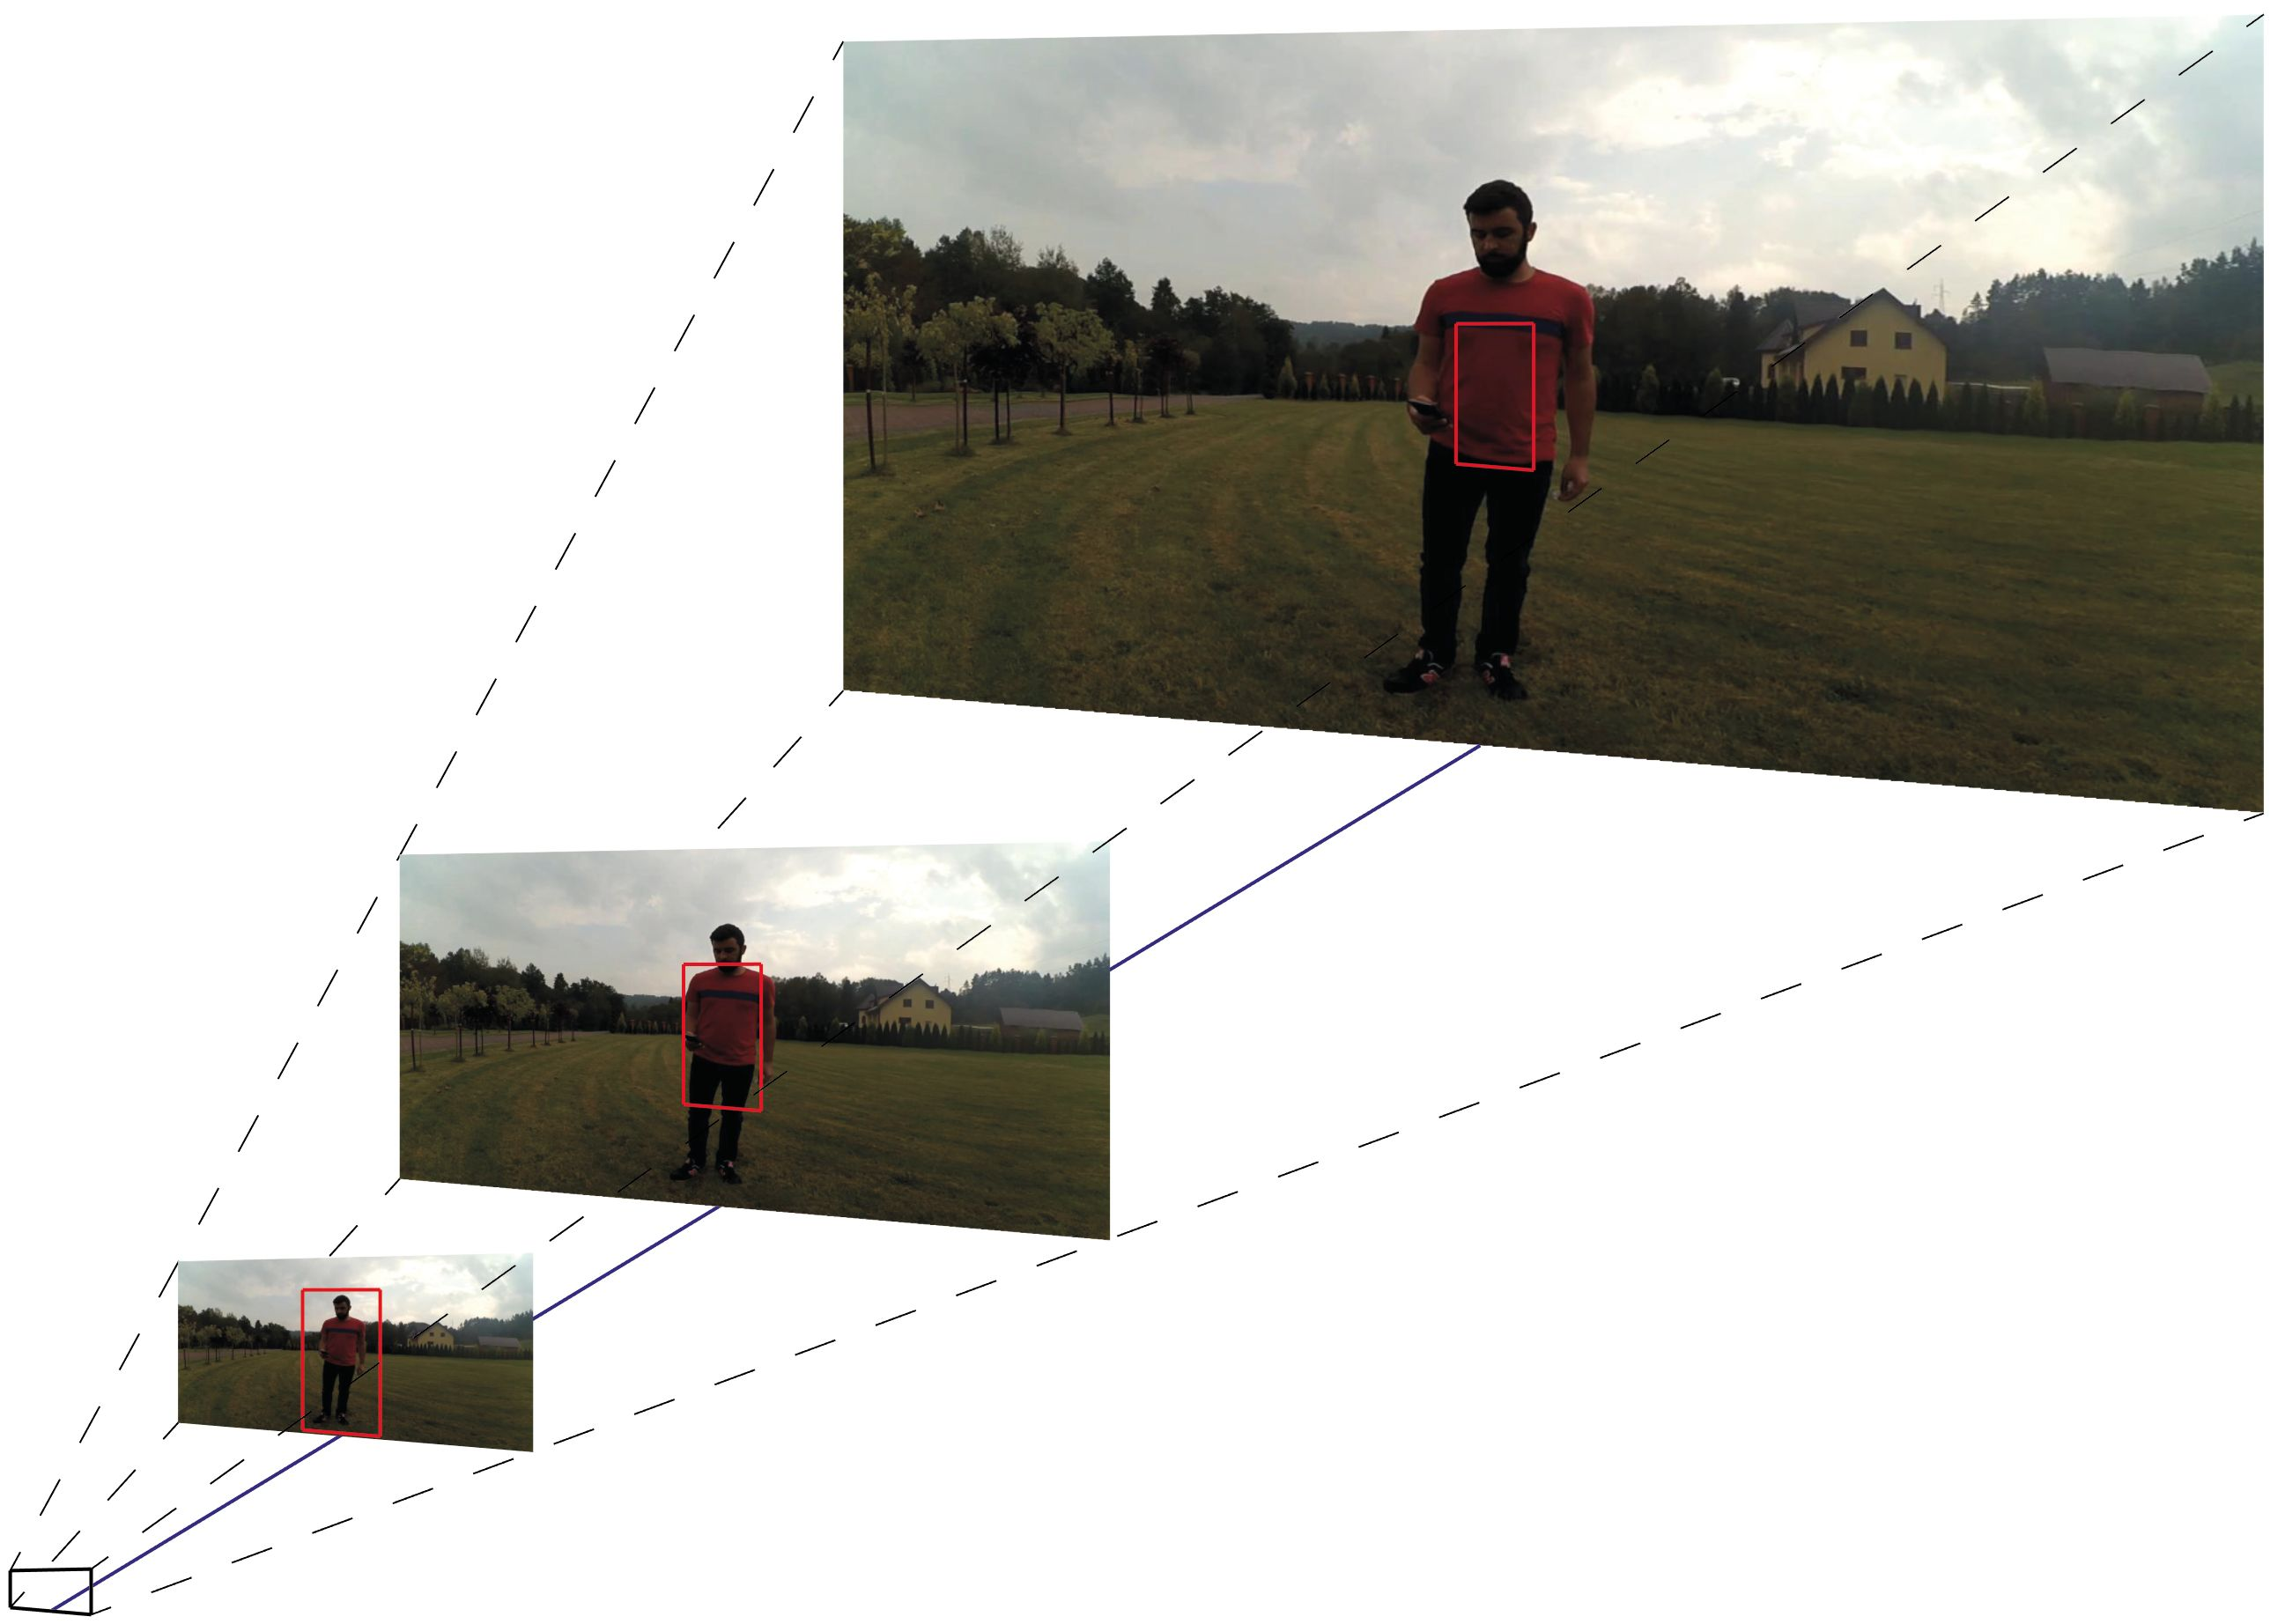
\includegraphics[width=15.5cm]{2_scaling.jpg}
	\caption{Skalowanie 1:1, 1:2 oraz 1:4 z naniesionym przykładowym oknem detekcji $128 \times 64$}
	\label{fig:HOG_image_examples}
\end{figure}
\newline
Widoczne na rysunku okno detekcji nasuwa wniosek, że osoba wykryta na oryginalnym obrazie będzie znacząco oddalona od kamery. Najbliżej rozpoznania postaci jest okno detekcji na obrazie przeskalowanym w stosunku 1:4.
Znając przybliżoną pozycję osoby wykrywanej przez takie okno na oryginale i stosując proste twierdzenie Talesa, można oszacować odległość. Opisuje to poniższy wzór:
\begin{equation}
\label{eq:scaling}
d_r=\frac{d_o}{s_c},
\end{equation}
gdzie $d_r$ to odległość rzeczywista, $d_o$ to odległość wykrytej osoby na obrazie oryginalnym (zmierzona), a $s_c$ to skala obrazu, na którym detekcja uzyskała najlepszy wynik (w postaci ułamkowej).

\subsection{Uczenie}
Aby detekcja mogła poprawnie działać, klasyfikator musi dysponować odpowiednimi parametrami. Uzyskuje się je na etapie uczenia, używając odpowiedniego zestawu danych.
Wzorując się na pracy Dalala oraz Triggsa, postanowiono skorzystać ze zbioru ponad 5000 obrazów udostępnionych przez twórców. Specyfikacja tego zestawu pozwala nauczyć klasyfikator rozpoznawać osoby na obrazie o wielkości $128\times 64$ pikseli. Wysokość przedstawionej osoby, wyrażona w pikselach, powinna oscylować wokół 95 ($\pm$ 5). \newline
Zgodnie z przyjętymi metodologiami, zestaw ten zawiera gotowy podział na próbki pozytywne i negatywne, dalej pogrupowane na zestaw trenujący oraz weryfikacyjny w stosunku zbliżonym do 70:30. Przykłady przedstawiono na ilustracji:

\begin{figure}[h]
	\centering
	\captionsetup{justification=centering,margin=1cm}
	\hspace*{1cm}
	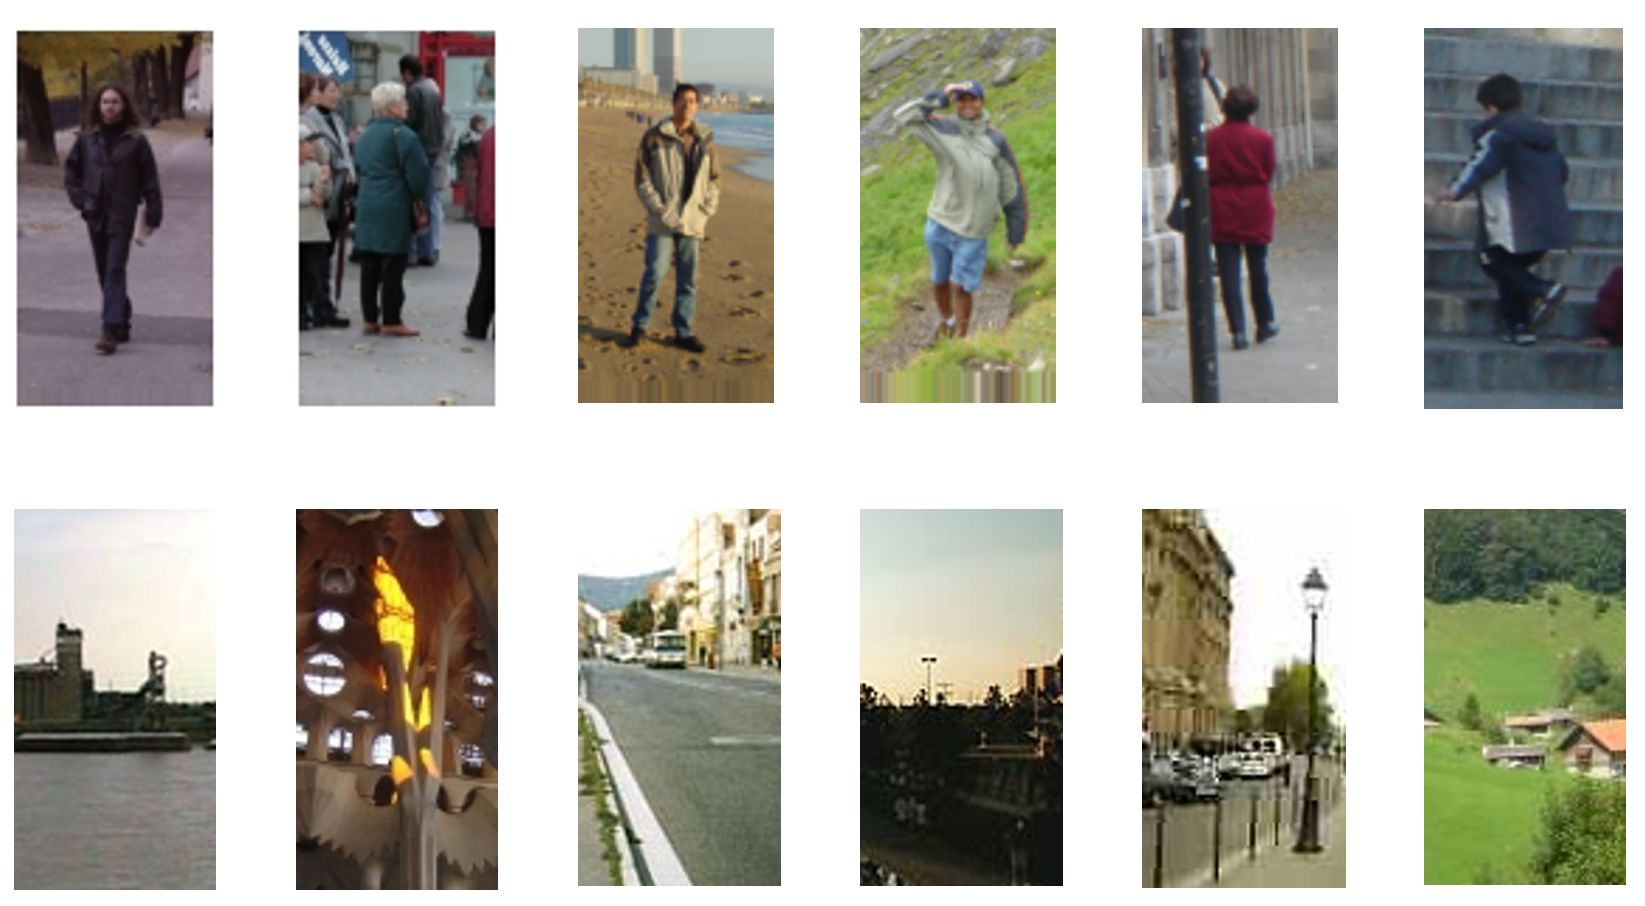
\includegraphics[width=14.5cm]{2_HOG_image_examples.jpg}
	\caption{Przykłady obrazów ze zbioru wykorzystanego przy uczeniu - po lewej dwie próbki pozytywne, po prawej dwie negatywne}
	\label{fig:HOG_image_examples}
\end{figure}
Wśród próbek pozytywnych połowa plików to duplikaty odwrócone horyzontalnie. Ma to zapewnić poprawne uwzględnienie cech usób niezależnie od orientacji względem kamery.

\subsection{Klasyfikacja}
\label{sec:klasyfikacja}
Etap ten jest stosunkowo prosty i stanowi główną zaletę klasyfikatora SVM. Wymaga bowiem wcześniejszego przeprowadzenia etapu uczenia, oraz dostarczenia wektora cech klasyfikowanego obiektu. Realizowane jest wówczas równanie:
\begin{equation}
\label{eq:HOG_classification}
\left.\begin{aligned} 
r=-\sum_{i=1}^{N}a_i(l_i+b_i)-c,
\end{aligned}\right.
\end{equation}
gdzie $a$, $b$ oraz $c$ to parametry hiperpłaszczyzny ($a$ i $b$ - wektory, $c$ - skalar), wszystkie wyliczone na etapie uczenia.
Jeśli $r>0$, detekcja wskazuje obiekt jako przynależący klasy, w przeciwnym wypadku go odrzuca.

